\documentclass[tikz,convert={outfile=\jobname.svg}]{standalone}
%\usetikzlibrary{...}% tikz package already loaded by 'tikz' option
\tikzset{dot/.style={draw,shape=circle,fill=black,scale=0.5}}
\usetikzlibrary{calc}
\begin{document}
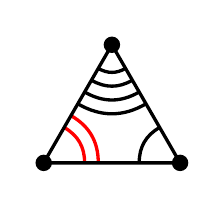
\begin{tikzpicture}[scale=1, very thick]
	\foreach \i in {0.2, 0.3, 0.4, 0.5} \draw ($(90:1)!\i!(90+120:1)$) to [out=-30,in=210] ($(90:1)!\i!(90-120:1)$);
	\foreach \i in {0.3, 0.4} \draw [red] ($(90+120:1)!\i!(90+120+120:1)$) to [out=90,in=-30] ($(90+120:1)!\i!(90:1)$);
	\foreach \i in {0.3} \draw ($(90+120+120:1)!\i!(90:1)$) to [out=210,in=90] ($(90+120+120:1)!\i!(90+120:1)$);
	
	\draw (90:1) -- (90+120:1) -- (90+120+120:1) -- cycle;
	\node [dot] at (90:1) {};
	\node [dot] at (90+120:1) {};
	\node [dot] at (90+120+120:1) {};
	
	\foreach \i in {90, 210, 330} \node at (\i:1.1) {};
\end{tikzpicture}
\end{document}
